\section{Pilastro $P27$}\label{sec:p27}

Come raffigurato in figura~\ref{fig:pianoPrimo} di pagina~\pageref{fig:pianoPrimo} il pilastro $P27$ è un pilastro centrale di dimensione $30\times 30\,cm$. Il calcolo dell'area di influenza del pilastro verrà eseguito per ogni piano dell'edificio. Si anticipa che piano secondo e copertura hanno lo stesso schema statico e perciò la medesima area di influenza.

\subsection{Copertura}

In copertura, e al piano secondo in maniera analoga, il pilastro $P27$ sorregge una trave in spessore di solaio a sei campate (di lunghezze diverse) e di conseguenza sulla trave è appoggiato, su cinque appoggi, il solaio. 

Una lunghezza di influenza sarà perciò definita dal pilastro rispetto alla trave, mentre l'altra sarà calcolata dallo schema statico del solaio appoggiato sulle travi. 

Nel primo caso, si assume che il vincolo estremo sul vano scala sia un appoggio semplice per via della non continuità dell'armatura. Con questa ipotesi si possono calcolare le due lunghezze di influenza (destra e sinistra) del pilastro.

\[
	\begin{cases}
		l_1^{dx} = 0.6\cdot l_{dx} = 0.6\cdot 5.65\,m = 3.39\,m\\
		l_1^{sx} = 0.5\cdot l_{sx} = 0.5\cdot 4.50\,m = 2.20\,m
	\end{cases}
\]
per un totale di
\[
	l_1 = 5.64\,m
\]

Nel secondo caso, si ha uno schema statico di quattro campate e cinque appoggi, per cui

\[
	\begin{cases}
		l_2^{up} = 0.6\cdot l_{up} = 0.6\cdot 5.00\,m = 3.00\,m\\
		l_2^{down} = 0.5\cdot l_{down} = 0.5\cdot 4.00\,m = 2.00\,m
	\end{cases}
\]
dove $up$ e $down$ è riferito rispetto alla figura~\ref{fig:infAreaCopertura}. La lunghezza totale della trave rispetto al solaio è di

\[
	l_2 = 5.00\,m
\]

Si deduce che l'area di influenza in copertura è

\[
	A_{inf}^{cop} = 5.64\cdot 5.00 = 28.20\,m^2
\]

\begin{figure}
	\centering
	\includegraphics[width=.6\textwidth]{p27_copertura}
	\caption{Area di influenza del pilastro $P27$ in copertura e secondo piano}
	\label{fig:infAreaCopertura}
\end{figure}

I carichi agenti in copertura sono:
\begin{itemize}
	\item carico della neve;
	\item azione del vento;
	\item carico di categoria H per sola manutenzione.
\end{itemize}
oltre ai pesi propri strutturali e non degli elementi.

Si deduce che, moltiplicando i carichi variabili per l'area di influenza trovata poco sopra, si ricava l'azione assiale che essi generano sul pilastro.

\[
	\begin{cases}
		N_{Q_s} = q_{neve} \cdot A_{inf}^{cop} = 2.41\cdot 28.20 = 67.96\,kN\\
		N_{Q_{CAT.H}} = q_{CAT.H} \cdot A_{inf}^{cop} = 0.5\cdot 28.20 = 14.10\,kN\\
		N_{Q_w} = p_{vento}\cdot A_{inf}^{cop} = \pm 0.138\cdot 28.20 = \pm 3.90\,kN
	\end{cases}
\]

Come già detto, si deve tenere conto dei pesi degli elementi strutturali; perciò

\begin{align*}
	\begin{cases}
		N_{G_1, trave} = 3.75\,\dfrac{kN}{m}\cdot(2.25 + 3.39)\,m = 21.15\,kN\\\\
		N_{G_1, solaio} = 3.60\,\dfrac{kN}{m^2}\cdot28.20\,m^2 = 101.52\,kN\\\\
		N_{G_2, solaio} = 2.84\,\dfrac{kN}{m^2}\cdot28.20\,m^2 = 80.09\,kN
	\end{cases}
\end{align*}
mentre il peso totale del pilastro è 

\begin{align*}
	N_{G_1, pilastro}^{tot} &= 25\,\dfrac{kN}{m^3}\cdot(0.30\cdot 0.30)\,m^2\cdot(2.75 +3.50+3.10+3.10-(0.04+0.16+0.05))\,m =\\&= 27.45\,kN
\end{align*}


Tenendo conto che la lunghezza di influenza del pilastro sulla trave è la medesima per tutti i piani si può definire l'azione totale generata dal peso della trave come

\[
	N_{G_1,trave}^{tot} = 4\cdot N_{G_1, trave} = 4 \cdot 21.15 = 84.60\,kN
\]

\subsection{Piano Secondo}
Il secondo piano può essere rappresentato con lo stesso schema statico della copertura; ne consegue che l'area di influenza è quella disegnata in figura~\ref{fig:infAreaCopertura} e vale
\[
	A_{inf}^{P2} = 28.20\,m^2
\]

Variano, ovviamente, i carichi che sono applicati; in particolare

\begin{align*}
	\begin{cases}
		N_{G_1, solaio} = 3.20\,\dfrac{kN}{m^2}\cdot28.20\,m^2 = 90.24\,kN\\\\
		N_{G_2, solaio} = 4.62\,\dfrac{kN}{m^2}\cdot28.20\,m^2 = 130.284\,kN\\\\
		N_{Q_{CAT.A}} = 2\,\dfrac{kN}{m^2}\cdot 28.20\,m^2 = 56.40\,kN
	\end{cases}
\end{align*}

\subsection{Piano Primo}

\begin{figure}
	\centering
	\includegraphics[width=.6\textwidth]{p27_pianoPrimo}
	\caption{Area di influenza del pilastro $P27$ al piano primo}
	\label{fig:infAreaPianoPrimo}
\end{figure}

Al piano primo la situzione cambia: mentre lato trave la lunghezza di influenza del pilastro è la stessa ($5.64\,m$), lato solaio si hanno delle differenze. Riportando in termini di schema statico, il solaio è appoggiato su tre appoggi ed ha, perciò, due campate. Ne consegue che le lunghezze di influenza, riportate graficamente in figura~\ref{fig:infAreaPianoPrimo}, sono calcolate come

\[
	\begin{cases}
		l_2^{up} = \dfrac{5}{8}\,cdot l = \dfrac{5}{8}\,cdot 5.00\,m = 3.125\,m\\
		l_2^{down} = \dfrac{5}{8}\,cdot l = \dfrac{5}{8}\,cdot 4.00\,m = 2.50\,m
	\end{cases}
\]
per un totale di
\[
	l_2 = 5.625\,m
\]
e perciò un'area di influenza del pilastro di
\[
	A_{inf}^{P1} = 5.64\,m \cdot 5.125\,m = 31.73\,m^2
\]

Le azioni di carichi e sovraccarichi sono

\begin{equation*}
	\begin{cases}
		N_{G_1, solaio} = 3.20\,\dfrac{kN}{m^2}\cdot31.73\,m^2 = 101.536\,kN\\\\
		N_{G_2, solaio} = 4.62\,\dfrac{kN}{m^2}\cdot31.73\,m^2 = 146.59\,kN\\\\
		N_{Q_{CAT.B2}} = 3\,\dfrac{kN}{m^2}\cdot 31.73\,m^2 = 95.17\,kN
	\end{cases}
\end{equation*}

\subsection{Piano Terra}
Il piano terra si differenzia leggermente dal piano precedente per l'area di influenza in quanto il solaio è formato da tre campate anziché due. Questo fa si che
\[
	l_1 = 5.64\,m
\]
mentre 
\[
	\begin{cases}
		l_2^{up} = 0.5\,cdot l = 0.5\,cdot 5.00\,m = 2.50\,m\\
		l_2^{down} = 0.6\,cdot l = 0.6\,cdot 4.00\,m = 2.40\,m
	\end{cases}
\]
per un totale di 
\[
	l_2 = 4.90\,m
\]

L'area di influenza del piano terra è di 
\[
	A_{inf}^{PT} = 5.64\,m \cdot 4.90\,m = 27.636\,m^2
\]

\begin{figure}
	\centering
	\includegraphics[width=.6\textwidth]{p27_pianoTerra}
	\caption{Area di influenza del pilastro $P27$ al piano terra}
	\label{fig:infAreaPianoTerra}
\end{figure}

Le azioni generate dai carichi agenti sul piano sono

\begin{equation*}
	\begin{cases}
		N_{G_1, solaio} = 3.0\,\dfrac{kN}{m^2}\cdot27.636\,m^2 = 99.50\,kN\\\\
		N_{G_2, solaio} = 4.62\,\dfrac{kN}{m^2}\cdot27.636\,m^2 = 127.68\,kN\\\\
		N_{Q_{CAT.D1}} = 4\,\dfrac{kN}{m^2}\cdot 27.636\,m^2 = 110.54\,kN
	\end{cases}
\end{equation*}

\subsection{Combinazione agli SLU}
Le combinazioni agli stati limite vengono eseguite come combinazione lineare (somma) degli SLU su ogni piano. In particolare, avendo in copertura tre carichi variabili (neve, vento e carico di categoria), la combinazione massima sarà quella fra le tre che da l'effetto massimo (generalmente il carico con valore più alto). Agli altri piani, al contrario, grava un solo carico variabile (quello di categoria); la combinazione agli SLU è unica.

In definitiva si ha

\begin{align*}
	N_{max}^{P27} =& \gamma_{G1_{SF}} \cdot (N_{G_1,pilastro}^{tot} + N_{G_1, trave}^{tot} + N_{G_1, solaio}^{cop} + N_{G_1, solaio}^{P2}+ N_{G_1, solaio}^{P1} + N_{G_1, solaio}^{PT}) +\\ &+\gamma_{G2_{SF}} \cdot (N_{G_2, solaio}^{cop} + N_{G_2, solaio}^{P2}+ N_{G_2, solaio}^{P1} + N_{G_2, solaio}^{PT}) +\\
	&+\gamma_{Q_{SF}}\cdot (N_{Q_s} + \psi_{w}\cdot N_{Q_w} + \psi_{CAT.H}\cdot N_{Q_{CAT.H}} + N_{Q_{CAT.A}} + N_{Q_{CAT.B2}} + N_{Q_{CAT.D1}}) =\\
	=& 1.3\cdot(86.40+27.45+101.52+90.24+101.536+99.50)+\\
	&+1.5\cdot(80.09+130.284+146.59+127.68)+\\
	&+1.5\cdot(67.96+0\cdot14.10+56.40+95.17+110.54+0.6\cdot3.90) =\\
	=& 1881.88\,kN
\end{align*}
\noindent
ricordando che i coefficienti di combinazioni sono quelli di tabella~\ref{tab:coeffPilastro}.

\begin{table}
	\centering
	\caption{Coefficienti dei carichi che agiscono sui pilastri}
	\label{tab:coeffPilastro}
	\begin{tabular}{lccccr}
		\toprule
		&$\gamma_{\MakeUppercase{sf}}$ & $\gamma_{\MakeUppercase{f}}$ &$\psi_{0i}$ &$\psi_{1i}$ &$\psi_{2i}$\\
		\midrule
		$G_1$ & $1.3$ &$1.0$\\
		$G_2$ &$1.5$ &$0.8$\\
		NEVE &$1.5$ &$0$ &$0.5$ &$0.2$ &$0$\\
		VENTO &$1.5$ &$0$ &$0.6$ & $0.2$&$0$\\
		CAT. H &$1.5$&$0$&$0$&$0$&$0$\\
		CAT. A &$1.5$&$0$&$0.7$&$0.5$&$0.3$\\
		CAT. B &$1.5$ &$0$ &$0.7$ &$0.5$ &$0.3$\\
		CAT. D &$1.5$ &$0$ &$0.7$ &$0.7$ &$0.6$\\
		\bottomrule
	\end{tabular}
\end{table}

\begin{figure}
	\centering
	\subfloat[\emph{Andamento dell'azione assiale massima sul pilastro $P27$}]{
	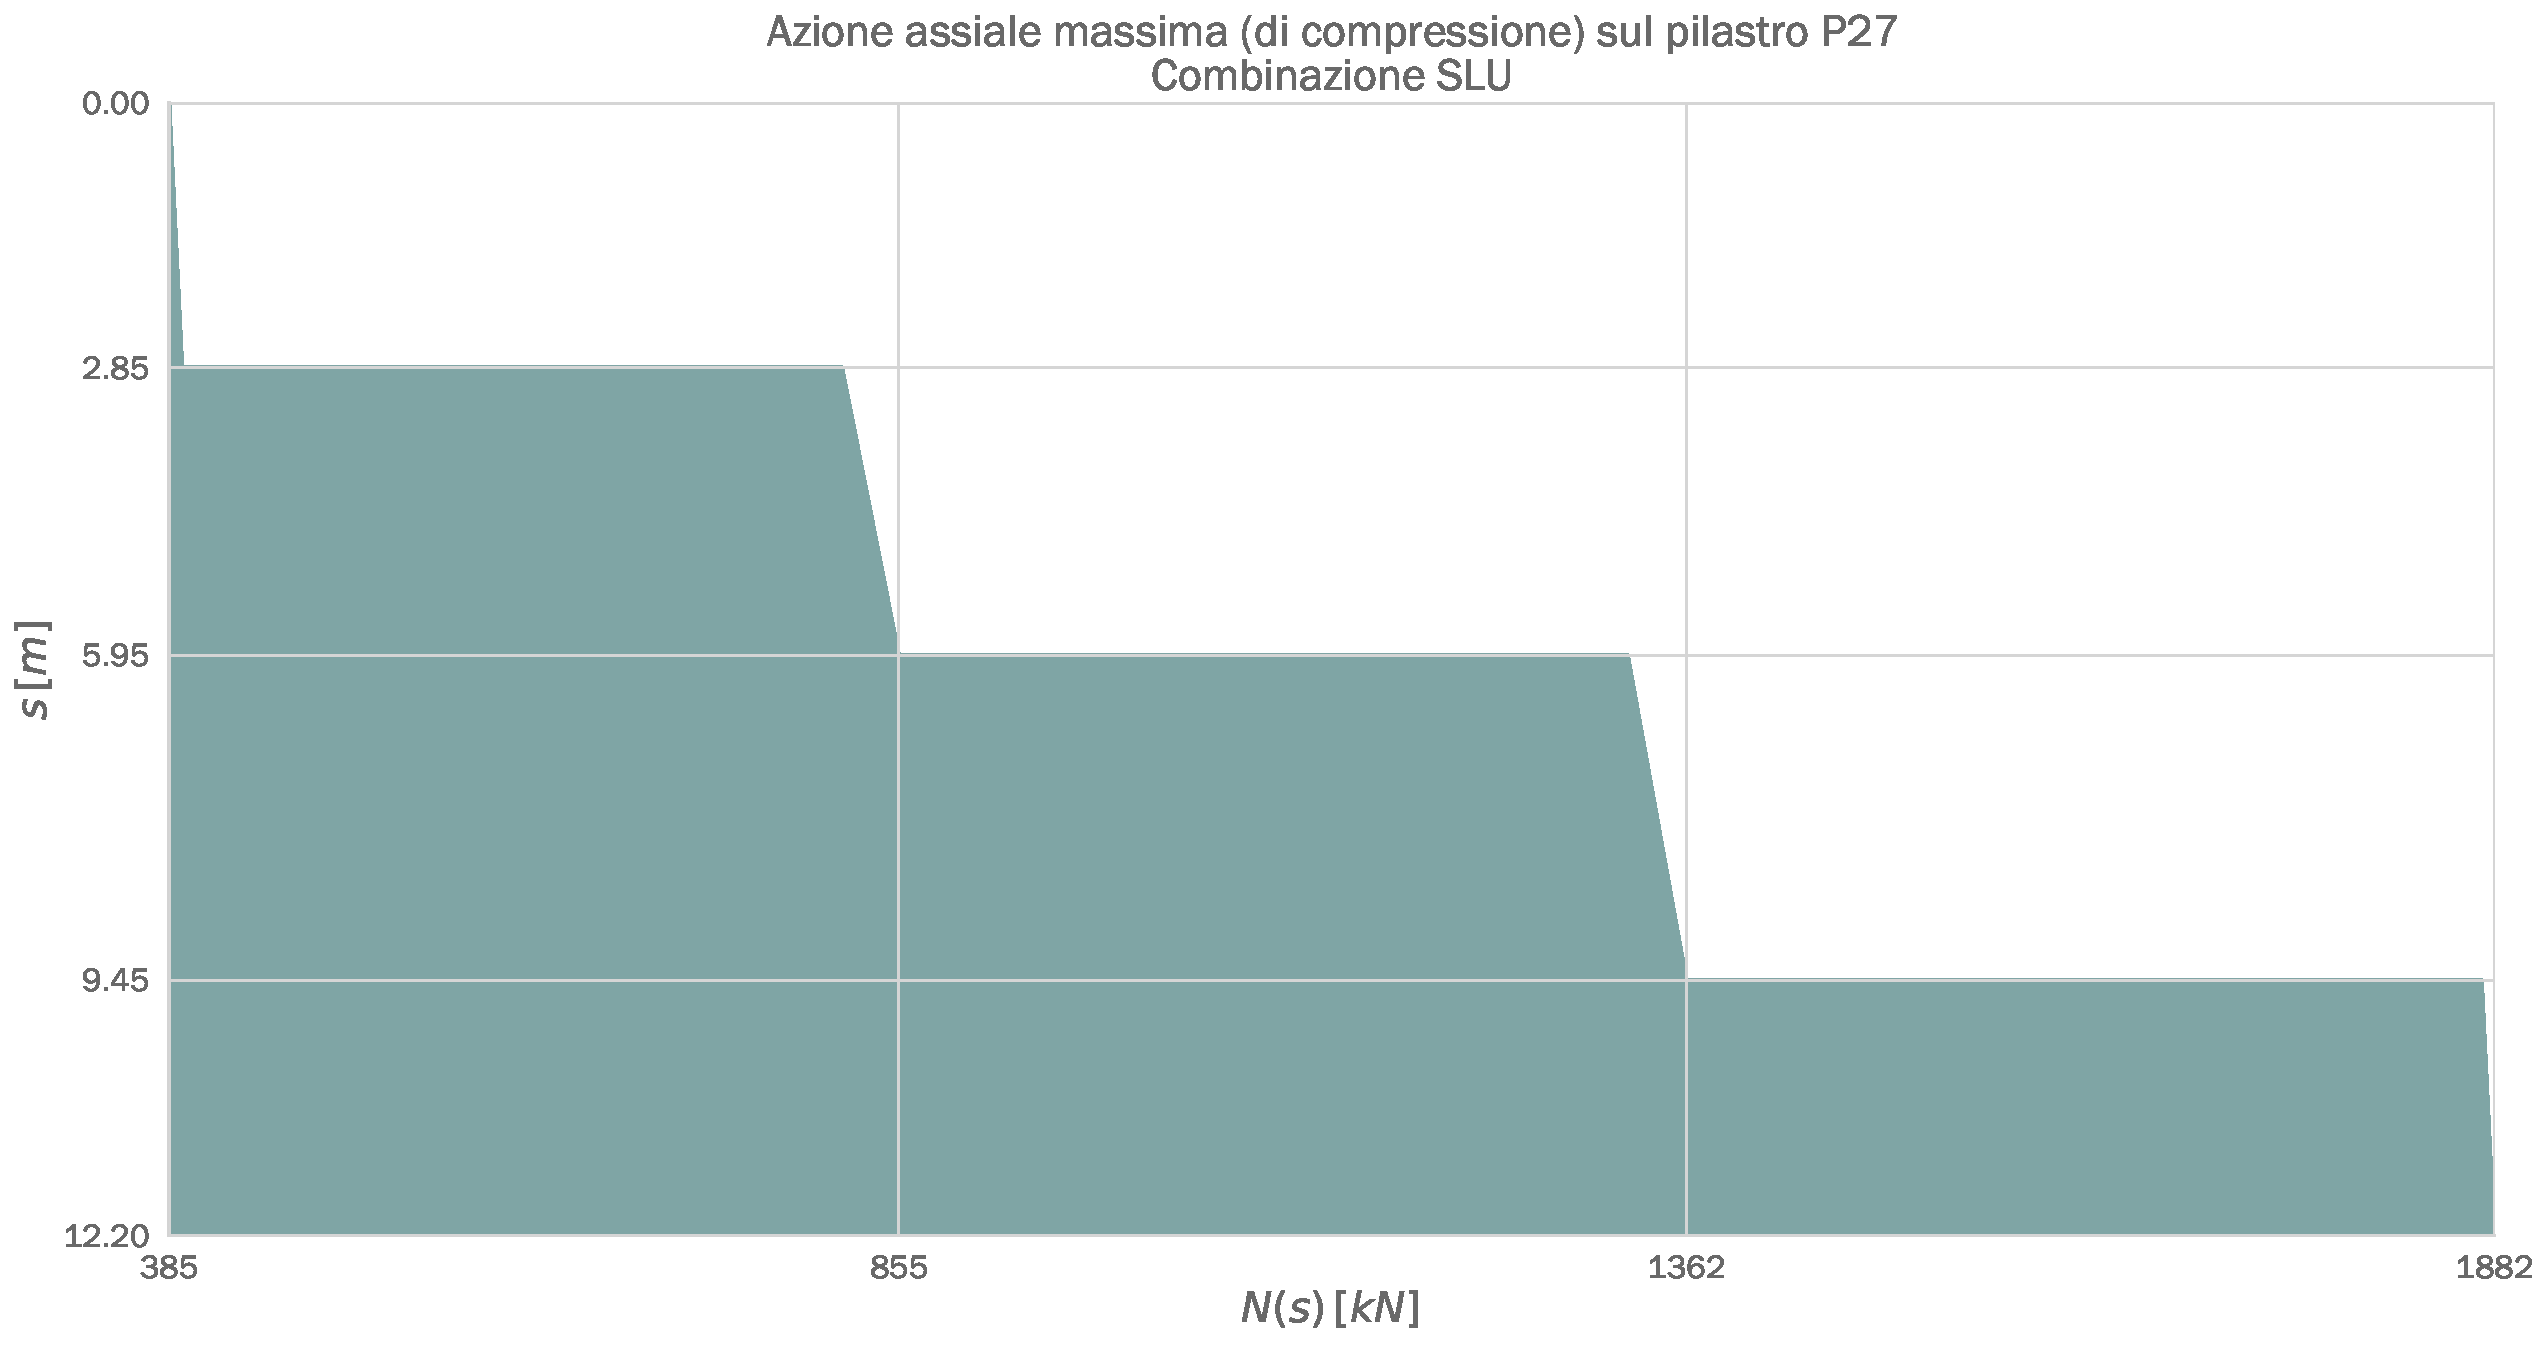
\includegraphics[width=.8\textwidth]{../../export/img/P27_maxAxialLoad_slu}}\\
	\subfloat[\emph{Andamento dell'azione assiale minima sul pilastro $P27$}]{
	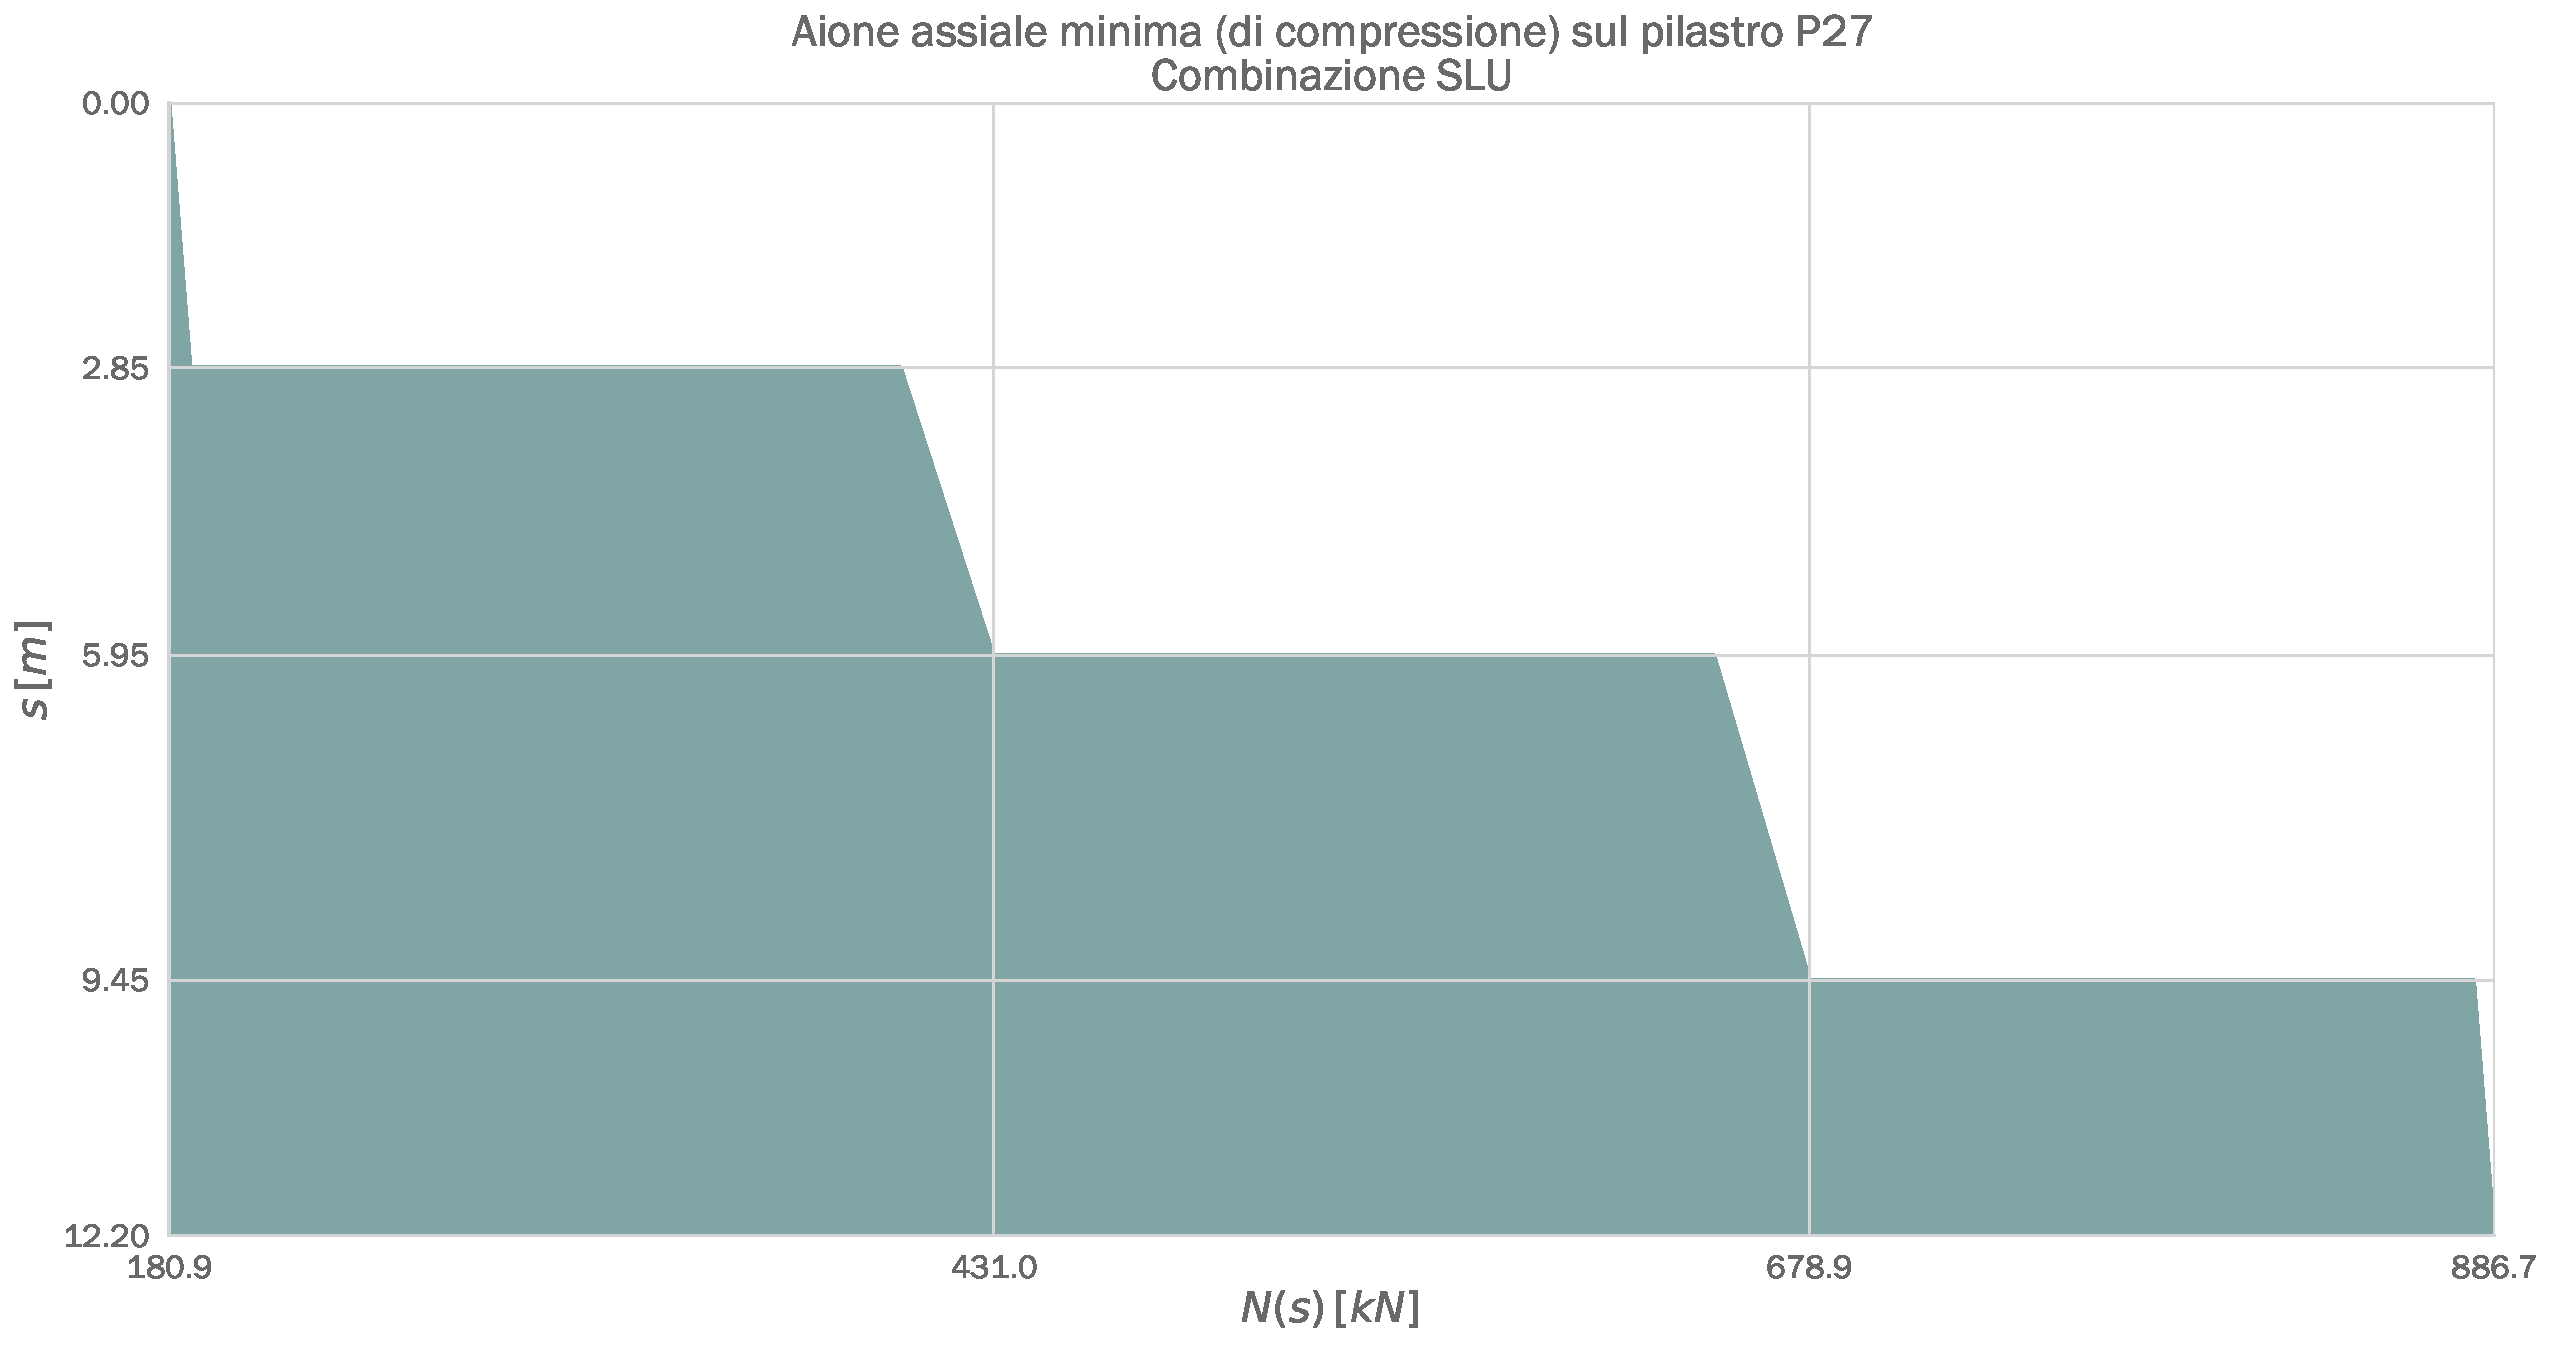
\includegraphics[width=.8\textwidth]{../../export/img/P27_minAxialLoad_slu}}
	\caption{Andamento delle azioni interne di compressione sul pilastro $P27$ in combinazione SLU}
	\label{fig:P27axialLoad_slu}
\end{figure}

Il valore minimo è

\begin{align*}
	N_{min}^{P27} =& 1.0\cdot(84.60+27.45+101.52+90.24+101.536+99.50)+\\
	&+0.8\cdot(80.09+130.284+146.59+127.68)+0 -1.5\cdot3.90 =\\
	=& 886.71\,kN
\end{align*}

L'andamento delle azioni di compressione massima e minima è riportato in figura~\ref{fig:P27axialLoad_slu}.

\subsection{Combinazione agli SLE rara}
Come ormai è noto, la combinazione rara non necessita di coefficienti di sicurezza; perciò

\begin{align*}
	N_{max}^{P27} =& (86.40+27.45+101.52+90.24+101.536+99.50)+\\
	&+(80.09+130.284+146.59+127.68)+\\
	&+(67.96+0\cdot14.10+56.40+95.17+110.54+0.6\cdot3.90) =\\
	=& 1321.90\,kN
\end{align*}

\begin{align*}
	N_{min}^{P27} =& (86.40+27.45+101.52+90.24+101.536+99.50)+\\
	&+(80.09+130.284+146.59+127.68)+\\
	&+(0.5\cdot67.96+0\cdot14.10+56.40+95.17+110.54-3.90) =\\
	=& 1281.68\,kN
\end{align*}

\begin{figure}
	\centering
	\subfloat[\emph{Andamento dell'azione assiale massima sul pilastro $P27$}]{
	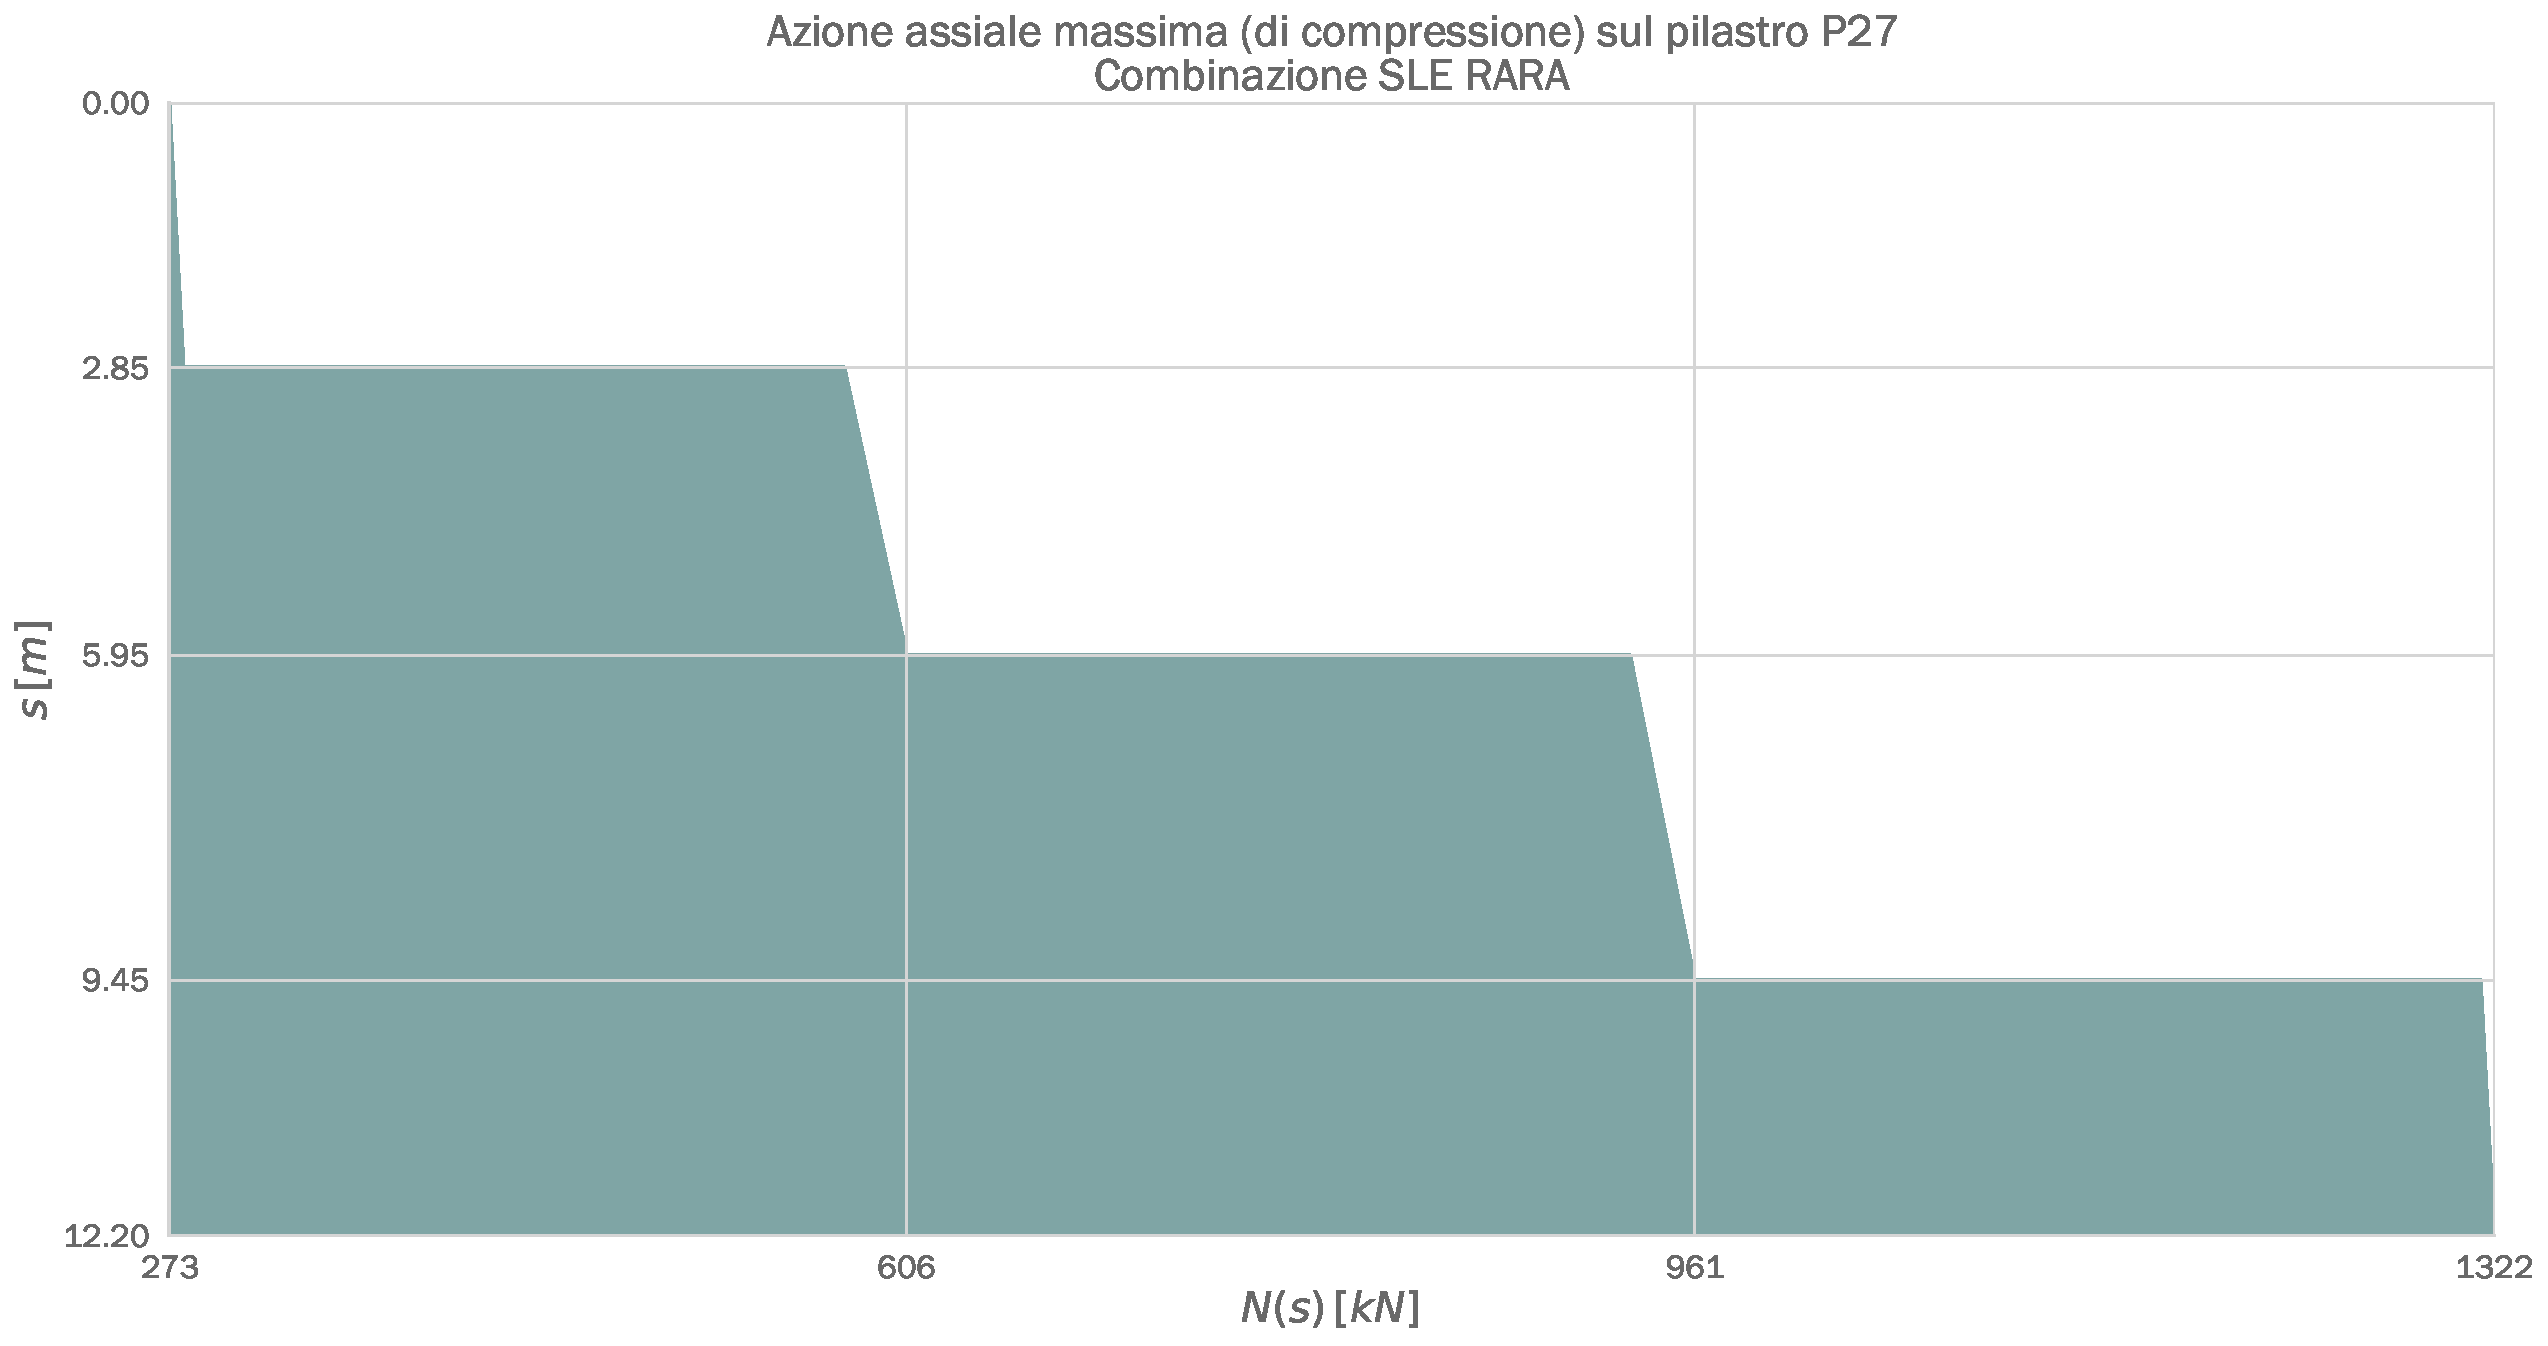
\includegraphics[width=.8\textwidth]{../../export/img/P27_maxAxialLoad_sleRara}}\\
	\subfloat[\emph{Andamento dell'azione assiale minima sul pilastro $P27$}]{
	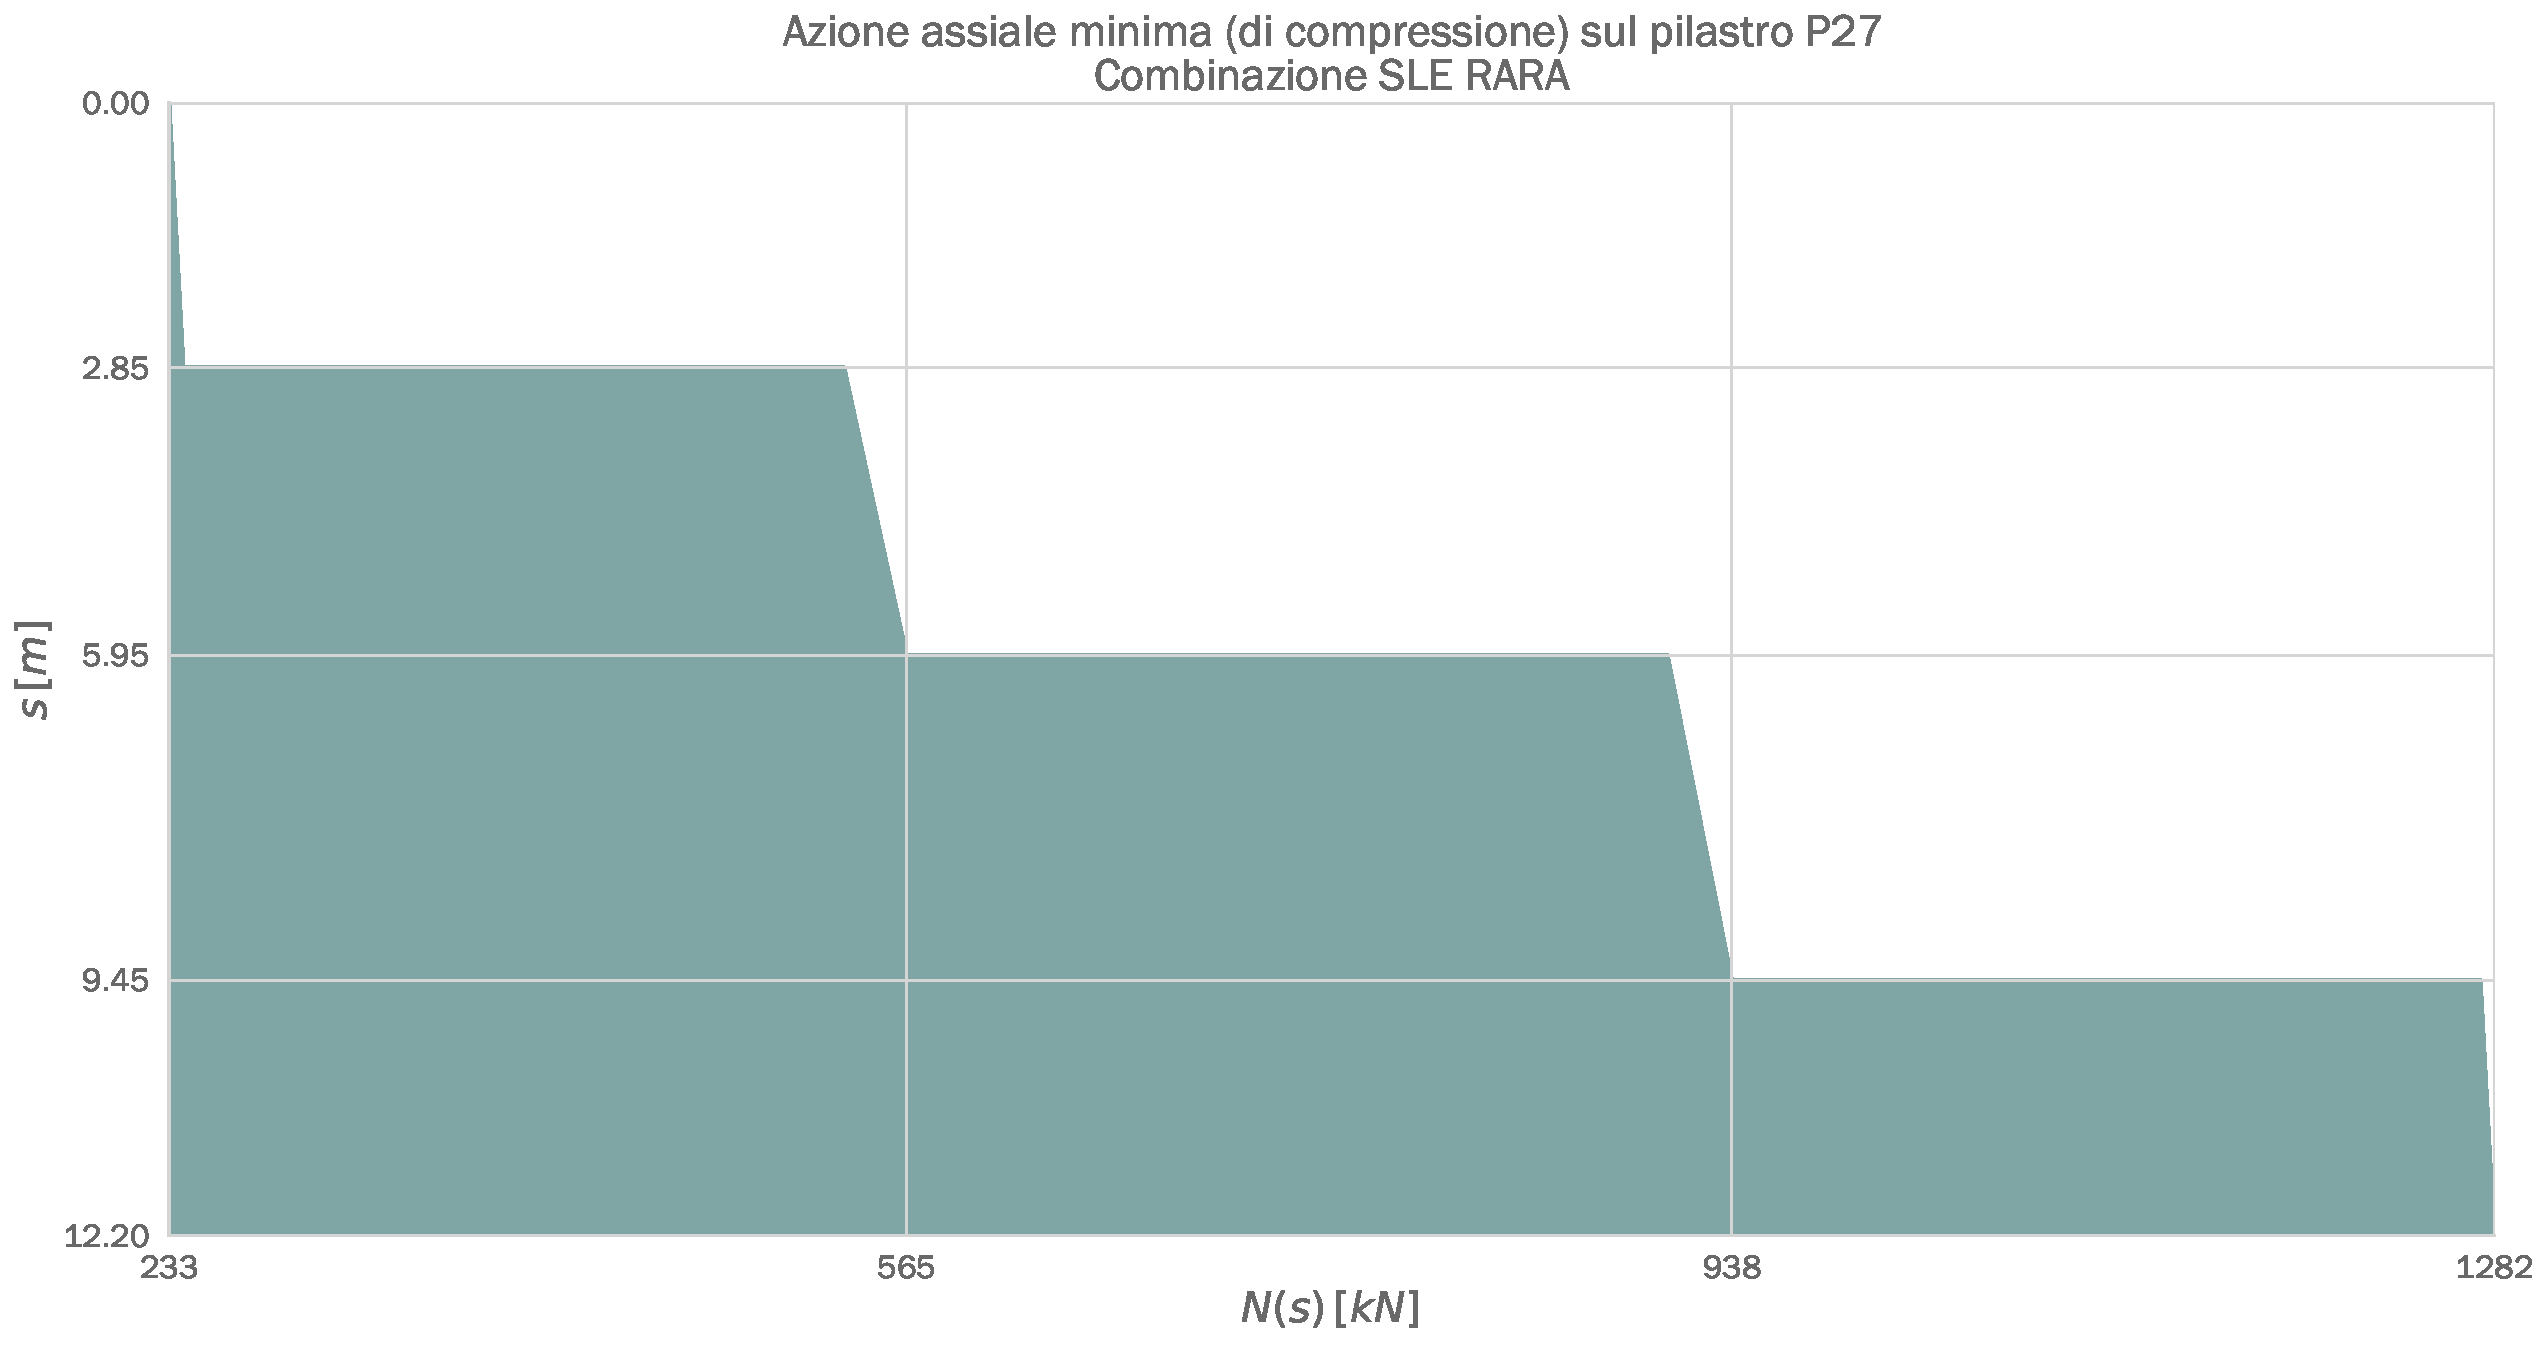
\includegraphics[width=.8\textwidth]{../../export/img/P27_minAxialLoad_sleRara}}
	\caption{Andamento delle azioni interne di compressione sul pilastro $P27$ in combinazione SLE rara}
	\label{fig:P27axialLoad_sleRara}
\end{figure}

\subsection{Combinazione agli SLE frequente}

\begin{align*}
	N_{max}^{P27} =& (86.40+27.45+101.52+90.24+101.536+99.50)+\\
	&+(80.09+130.284+146.59+127.68)+\\	&+(0.2\cdot67.96+0\cdot14.10+0.5\cdot56.40+0.5\cdot95.17+0.7\cdot110.54+0\cdot3.90) =\\
	=& 1156.245\,kN
\end{align*}

\begin{align*}
	N_{min}^{P27} =& (86.40+27.45+101.52+90.24+101.536+99.50)+\\
	&+(80.09+130.284+146.59+127.68)+\\	&+(0\cdot67.96+0\cdot14.10+0.3\cdot56.40+0.3\cdot95.17+0.3\cdot110.54-0.2\cdot3.90) =\\
	=& 1100.505\,kN
\end{align*}

\begin{figure}
	\centering
	\subfloat[\emph{Andamento dell'azione assiale massima sul pilastro $P27$}]{
	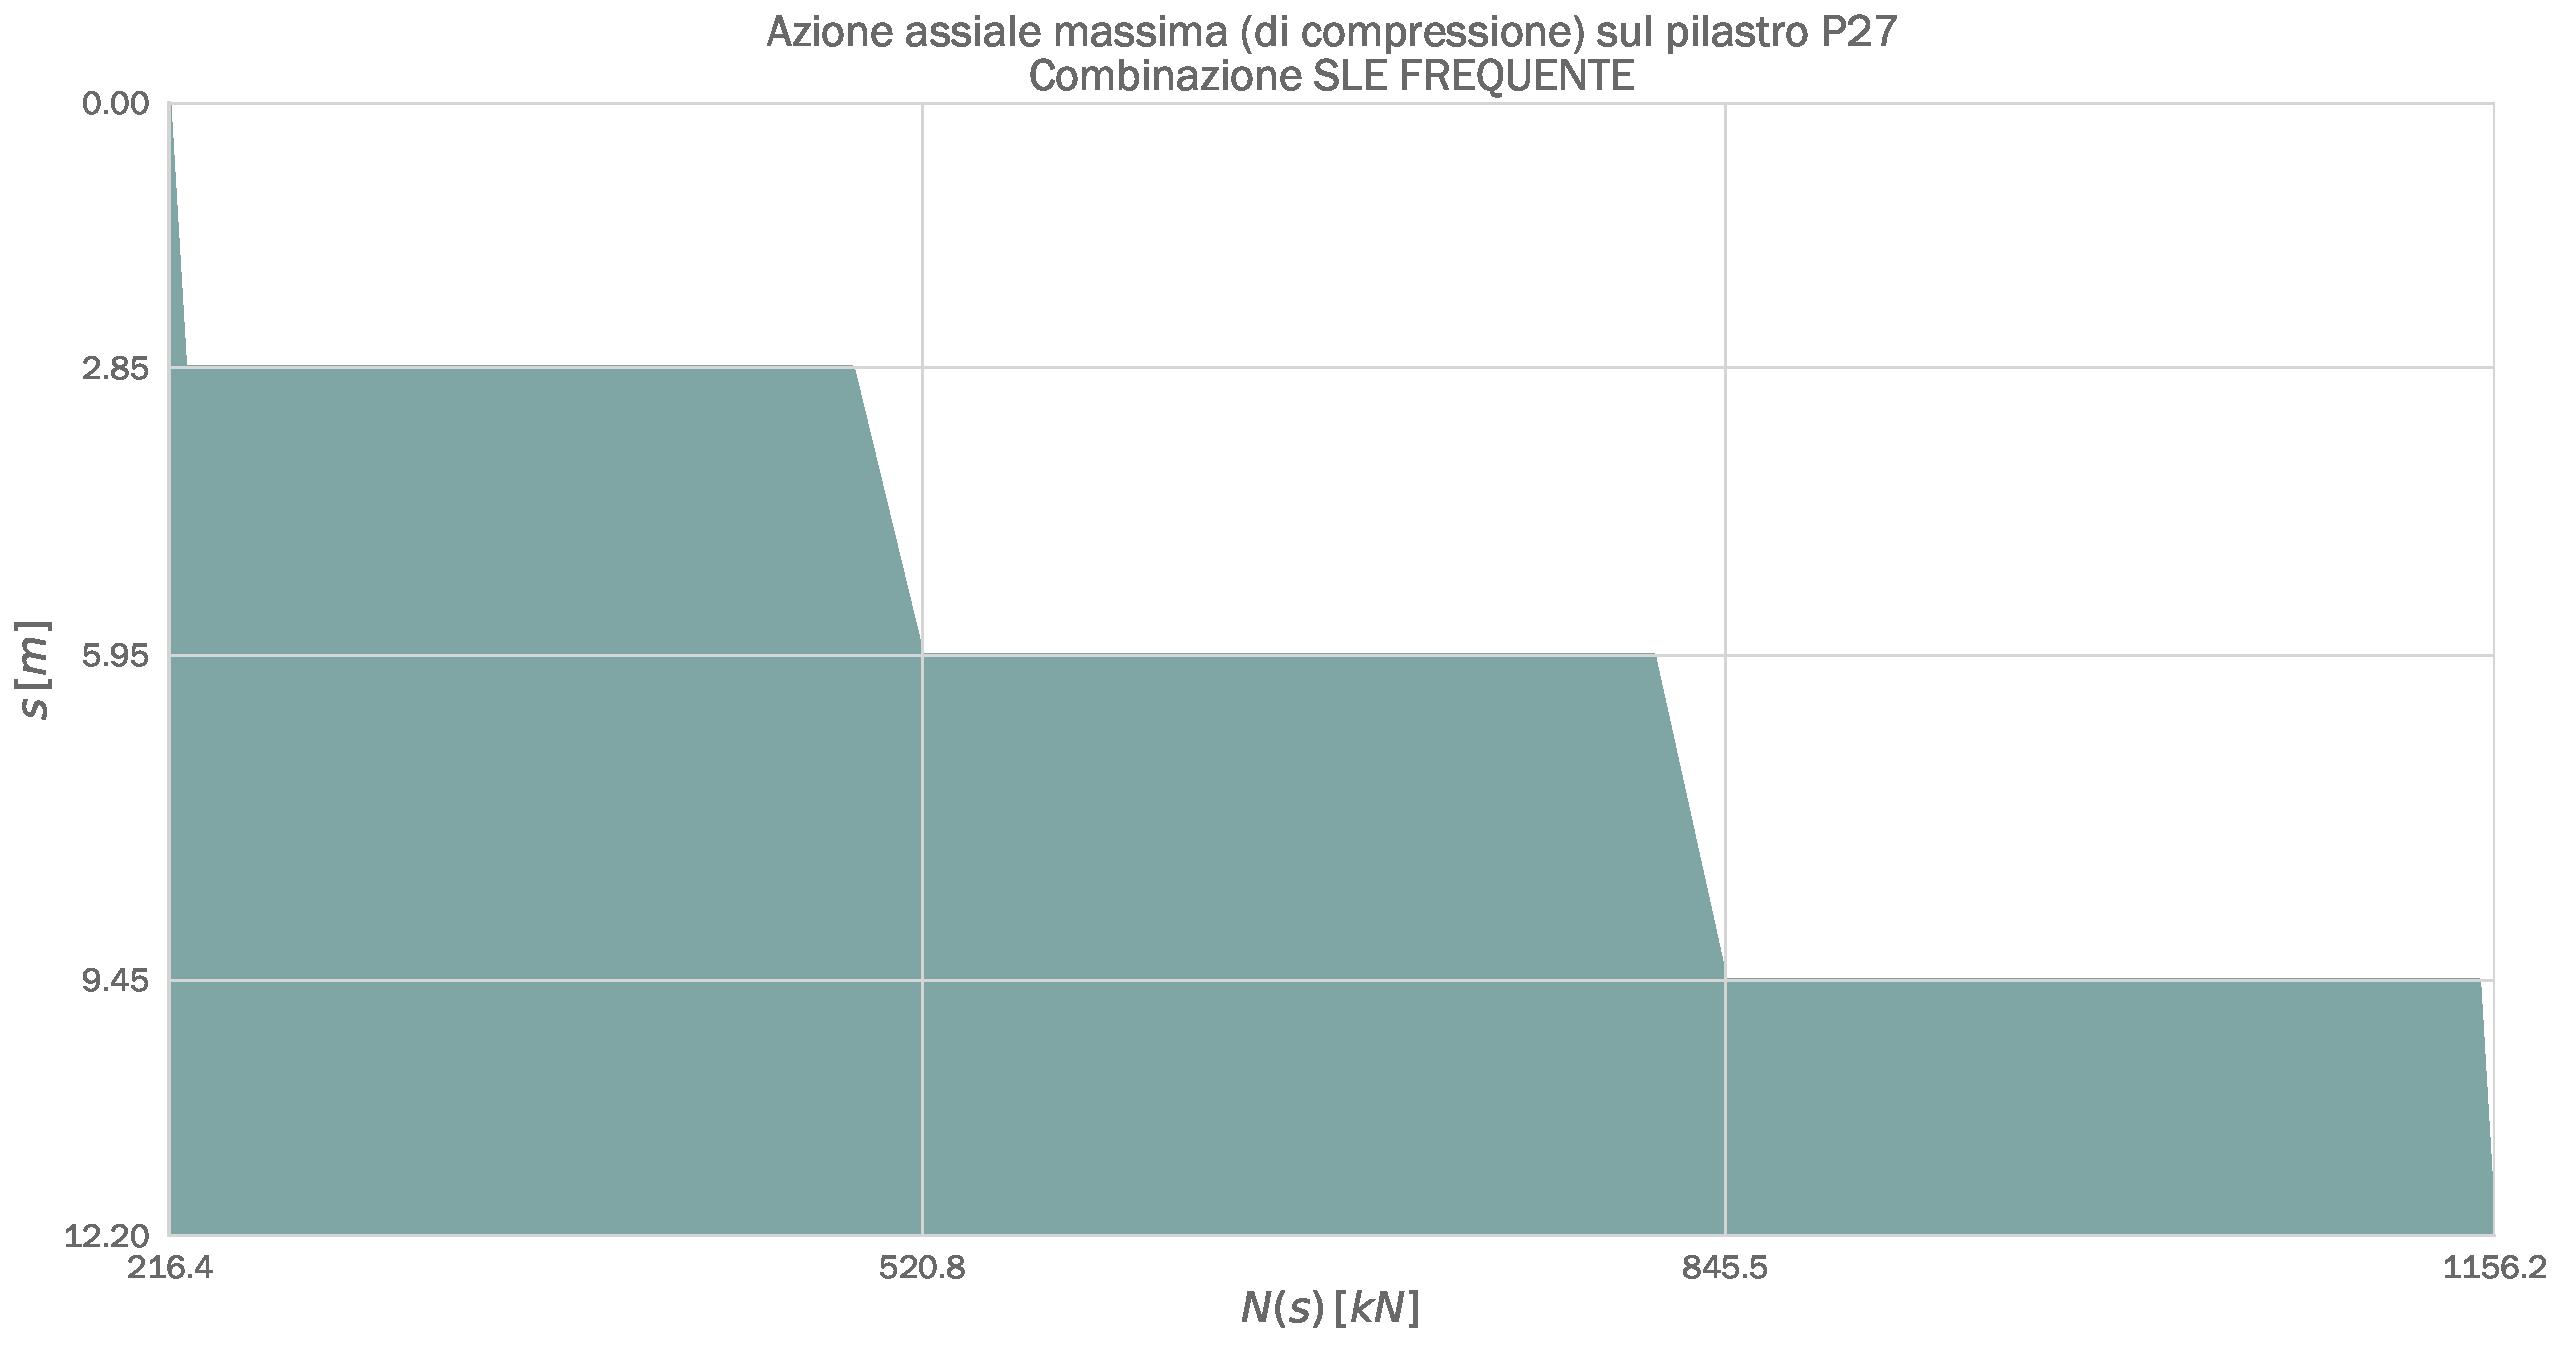
\includegraphics[width=.8\textwidth]{../../export/img/P27_maxAxialLoad_sleFreq}}\\
	\subfloat[\emph{Andamento dell'azione assiale minima sul pilastro $P27$}]{
	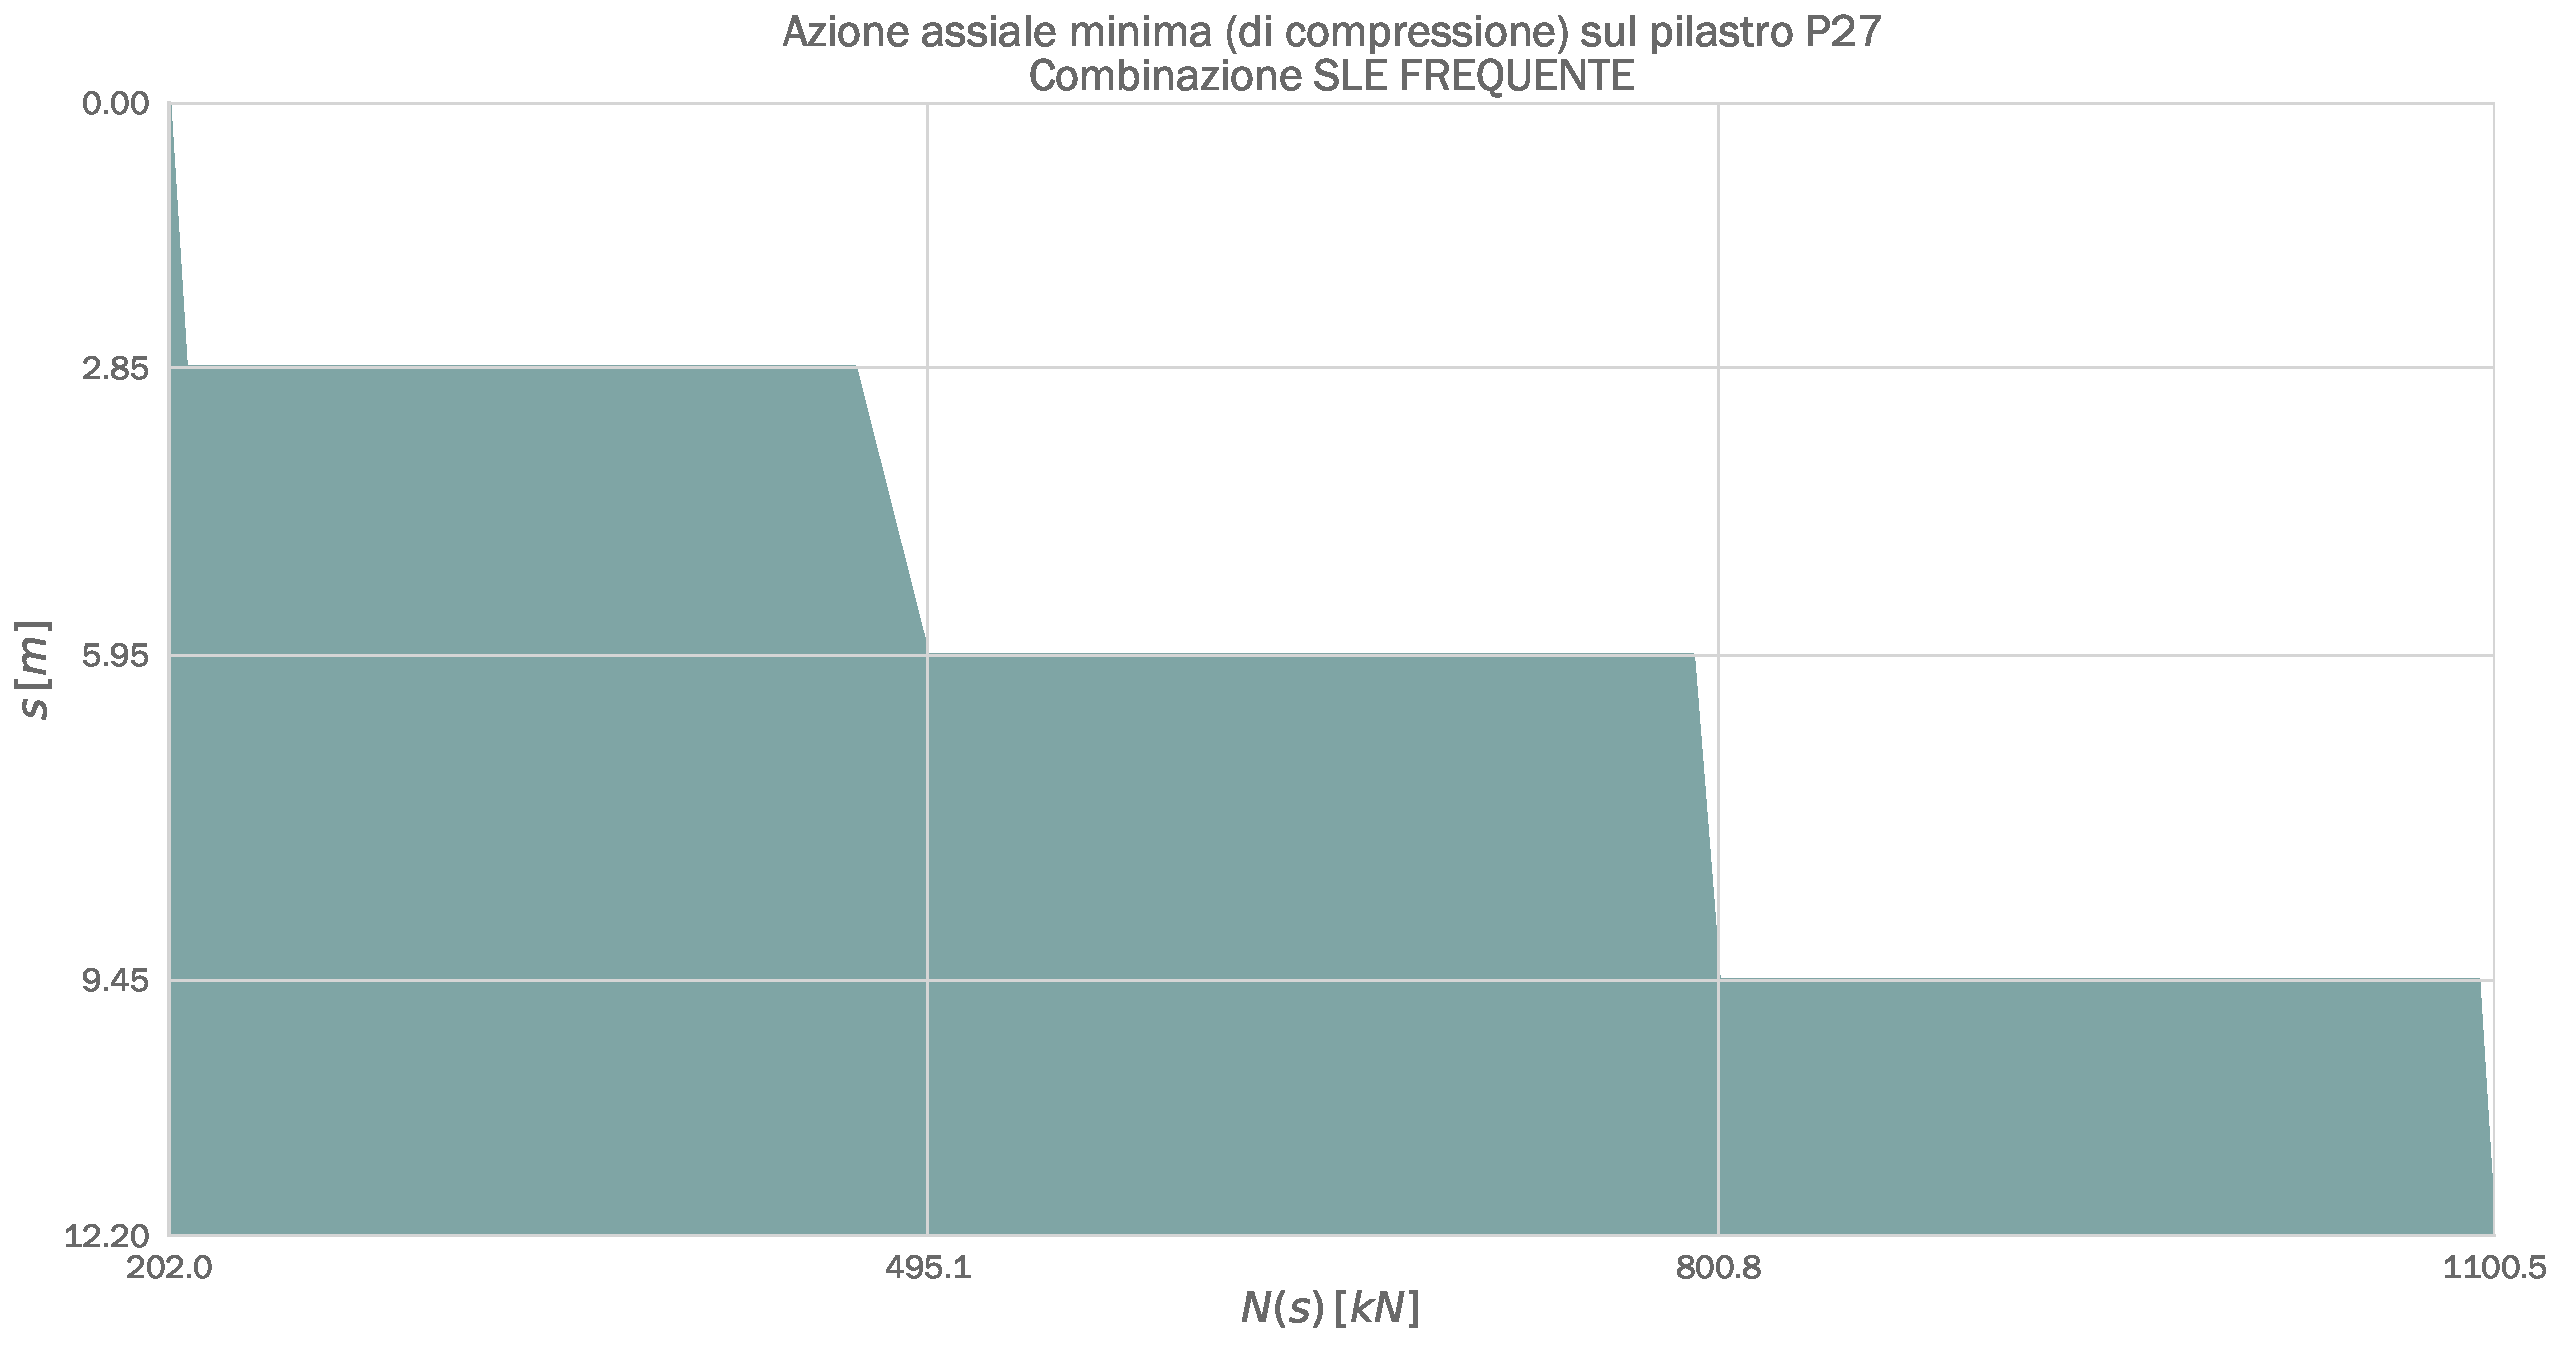
\includegraphics[width=.8\textwidth]{../../export/img/P27_minAxialLoad_sleFreq}}
	\caption{Andamento delle azioni interne di compressione sul pilastro $P27$ in combinazione SLE frequente}
	\label{fig:P27axialLoad_sleFreq}
\end{figure}

\subsection{Combinazione agli SLE quasi permanente}
Per gli SLE quasi permanente viene calcolata una sola configurazione di carichi, non essendoci combinazioni.

\begin{align*}
	N^{P27} =& (86.40+27.45+101.52+90.24+101.536+99.50)+\\
	&+(80.09+130.284+146.59+127.68)+\\	&+(0\cdot67.96+0\cdot14.10+0.3\cdot56.40+0.3\cdot95.17+0.6\cdot110.54+0\cdot3.90) =\\
	=& 1101.285\,kN
\end{align*}


\begin{figure}
	\centering
	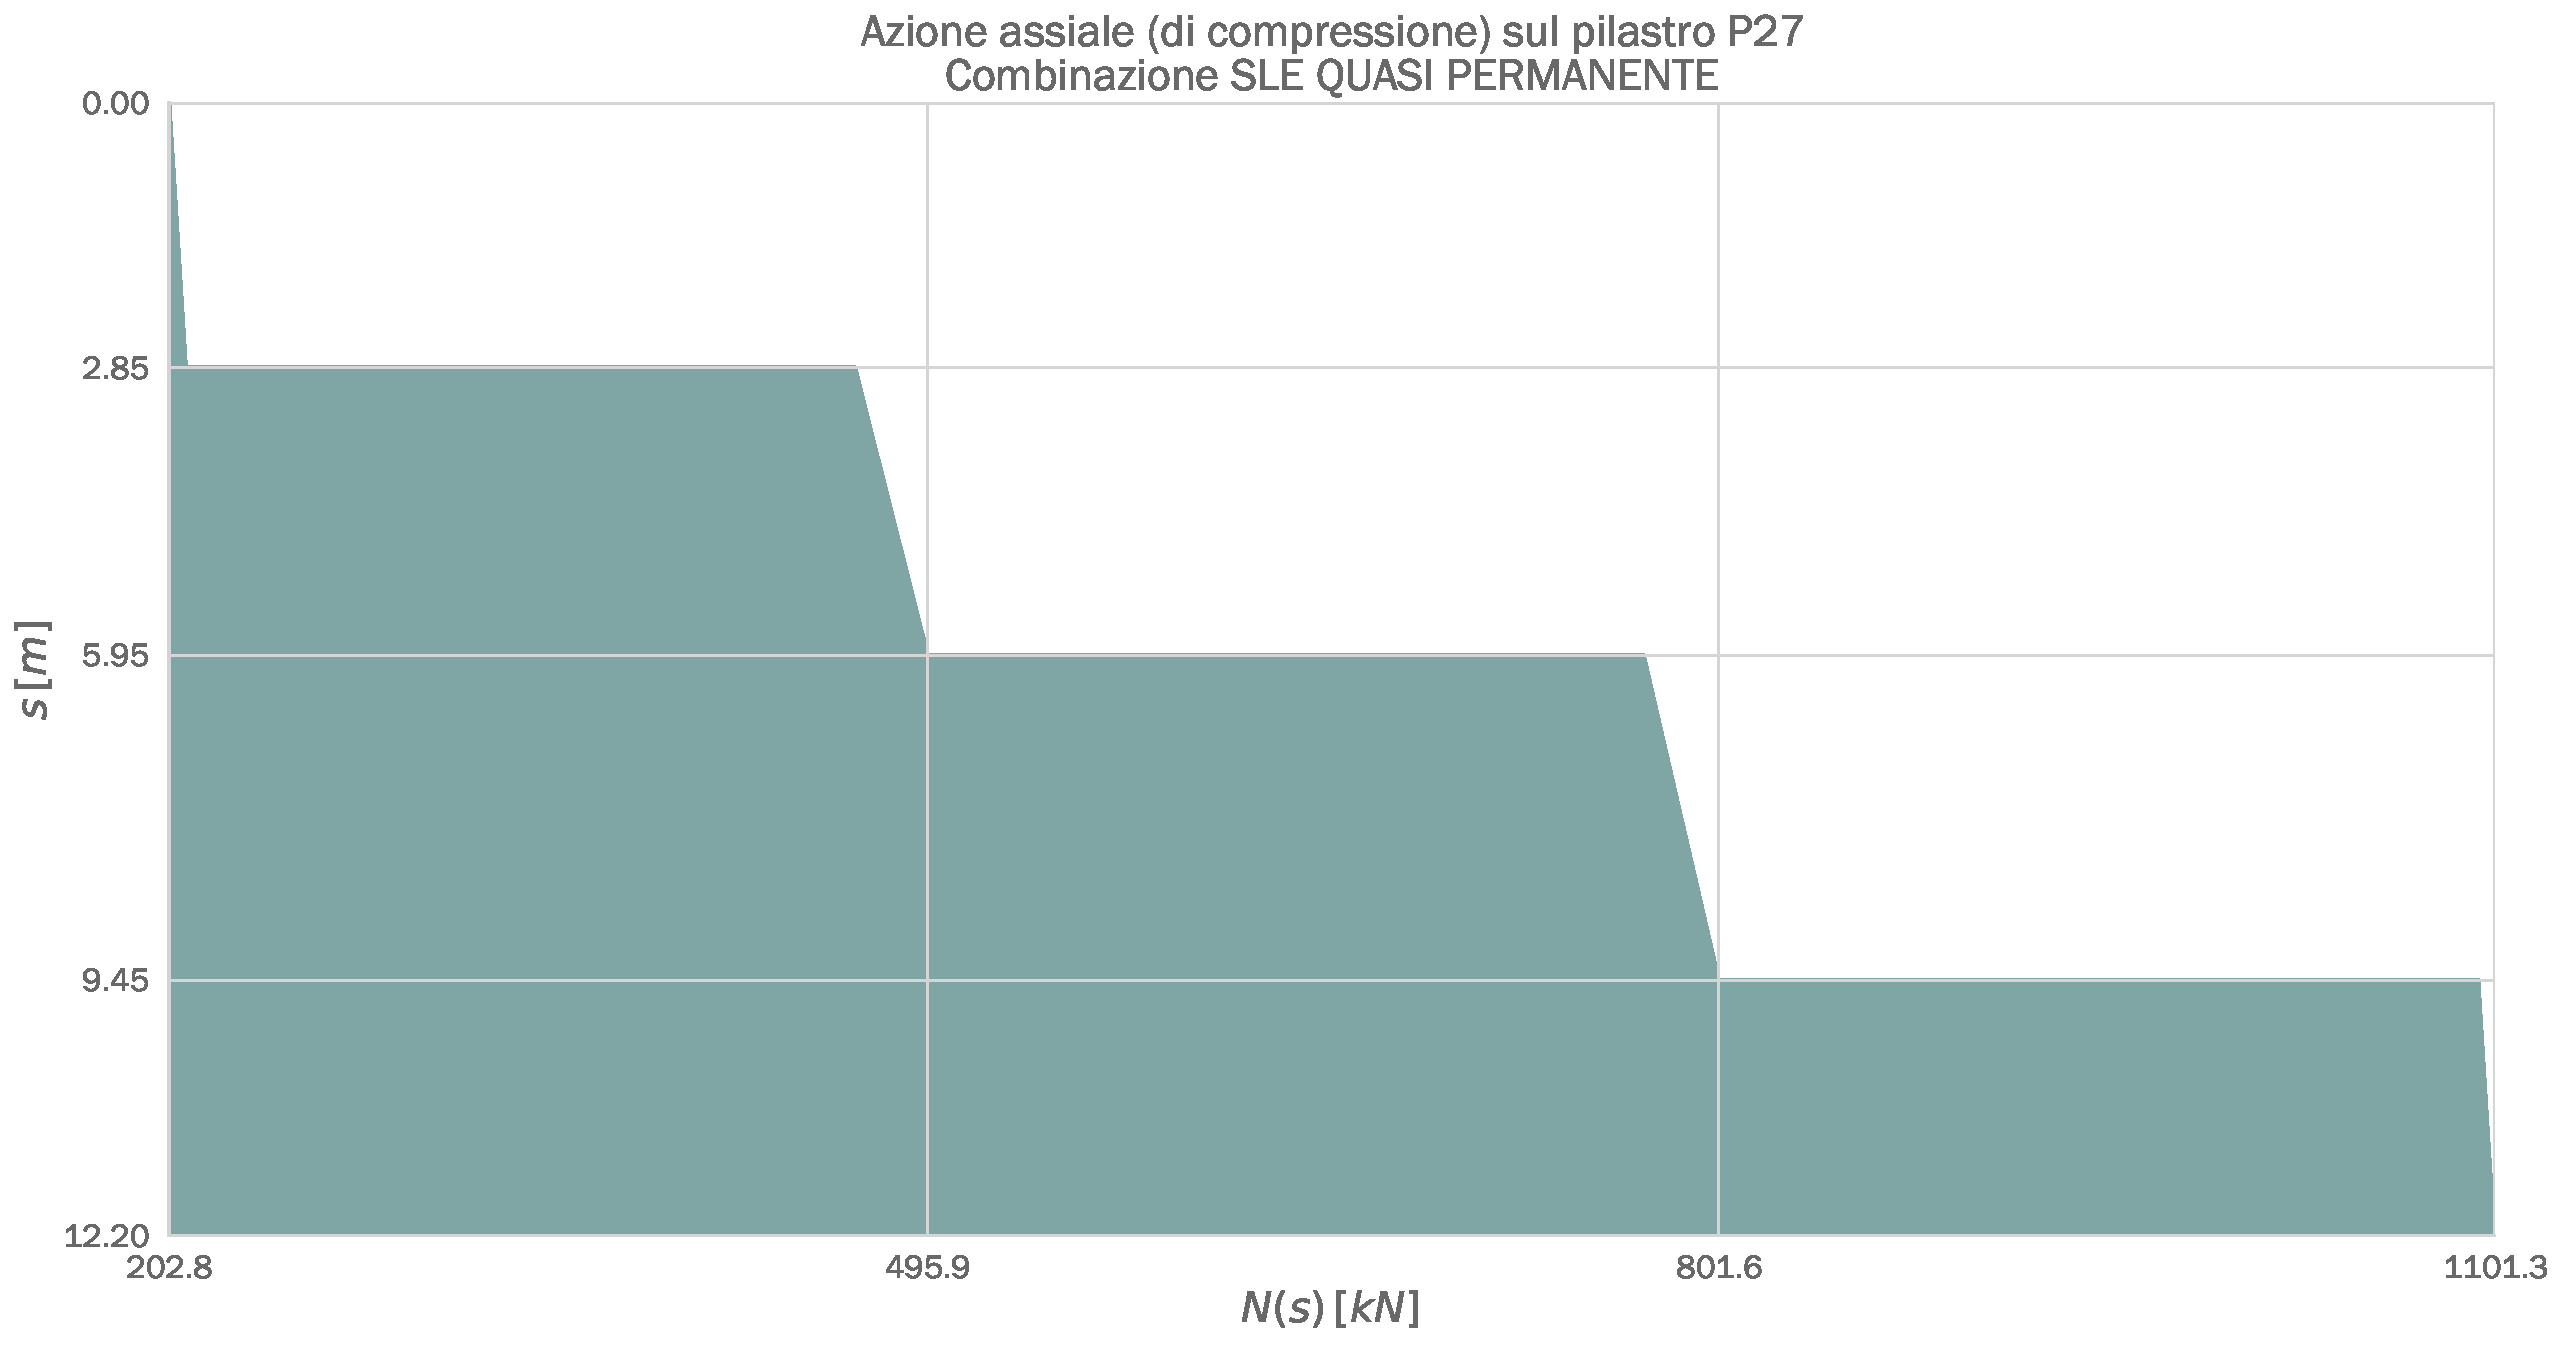
\includegraphics[width=.8\textwidth]{../../export/img/P27_axialLoad_sleQP}
	\caption{Andamento dell'azione interna di compressione sul pilastro $P27$ in combinazione SLE quasi permanente}
	\label{fig:P27axialLoad_sleQP}
\end{figure}

È così conclusa l'analisi delle sollecitazioni per il pilastro $P27$. 

Seguono i calcoli per il pilastro $P36$.
\cleardoublepage

%-----------------------------------------------
